% PROOF OF CONCEPT
In the previous sections it was demonstrated that likelihood functions can be indeed spectrally expanded and that the posterior density with its moments can be computed accordingly.
For low-dimensional problems the SLE convergence behavior up to a high degree was studied by monitoring the LOO error.
It was shown that the expansion error can be arbitrarily reduced by increasing the order of the expansion and adding samples to the experimental design.
% HIGHER DIMENSIONAL
While this is reassuring to know, it does not help in solving higher-dimensional problems
for which the computation of high-order expansions is exacerbated by the curse of dimensionality.
Hence, now we want to investigate the applicability of SLEs and aSLEs in an inverse problem of moderate dimension.
\par % PROBLEM SETUP
An IHCP in two spatial dimensions with six unknown conductivities is considered in this section.
The setup of the problem is shown in \cref{fig:JCP:Thermal:HeatConduction}.
The \(\dimParam = 6\) unknown conductivities \(\bm{\kappa} = (\kappa_1,\ldots,\kappa_6)^\top\) are inferred
with \(\dimData = 20\) noisy measurements \(\bm{T} = (T_{1},\ldots,T_{20})^\top\) of the temperature field \(\perfect{T}\).
% EXPERIMENTAL SETUP
We set \(\kappa_0 = \unit[30]{W/m/K}\) and \(\bm{\kappa} = \unit[(20,24,\ldots,40)^\top]{W/m/K}\).
The prior is set to a multivariate lognormal distribution \(\pi(\bm{\kappa}) = \prod_{i=1}^6 \pi(\kappa_i)\) with independent marginals
\(\pi(\kappa_i) = \mathcal{LN}( \kappa_i \cond \mu_0,\sigma_0^2)\) with \(\mu_0 = \unit[30]{W/m/K}\) and \(\sigma_0 = \unit[6]{W/m/K}\).
These parameters describe the mean \(\mu_0 = \mathds{E}[\kappa_i]\) and standard deviation \(\sigma_0 = \mathrm{Std}[\kappa_i]\) of the lognormal prior.
They are related to the parameters of the associated normal distribution \(\mathcal{N}( \log(\kappa_i) \cond \lambda_0,\varsigma_0^2)\)
via \(\mu_0 = \exp(\lambda_0 + \varsigma_0^2 / 2)\) and \(\sigma_0^2 = (\exp(\varsigma_0^2) - 1) \exp(2 \lambda_0 + \varsigma_0^2)\).
Otherwise than that, the problem setup is exactly as described in the previous section,
i.e.\ the likelihood function is given as \(\mathcal{L}(\bm{\kappa}) = \mathcal{N}(\bm{T} \cond \mathcal{M}(\bm{\kappa}),\bm{\Sigma})\).
In accordance with this setup, in the following synthetic data are simulated and analyzed in order to compute
the joint posterior \(\pi(\bm{\kappa} \cond \bm{T}) = \scale^{-1} \mathcal{L}(\bm{\kappa}) \pi(\bm{\kappa})\).
% FIGURE: PDE
\begin{figure}[htbp]
  \centering
  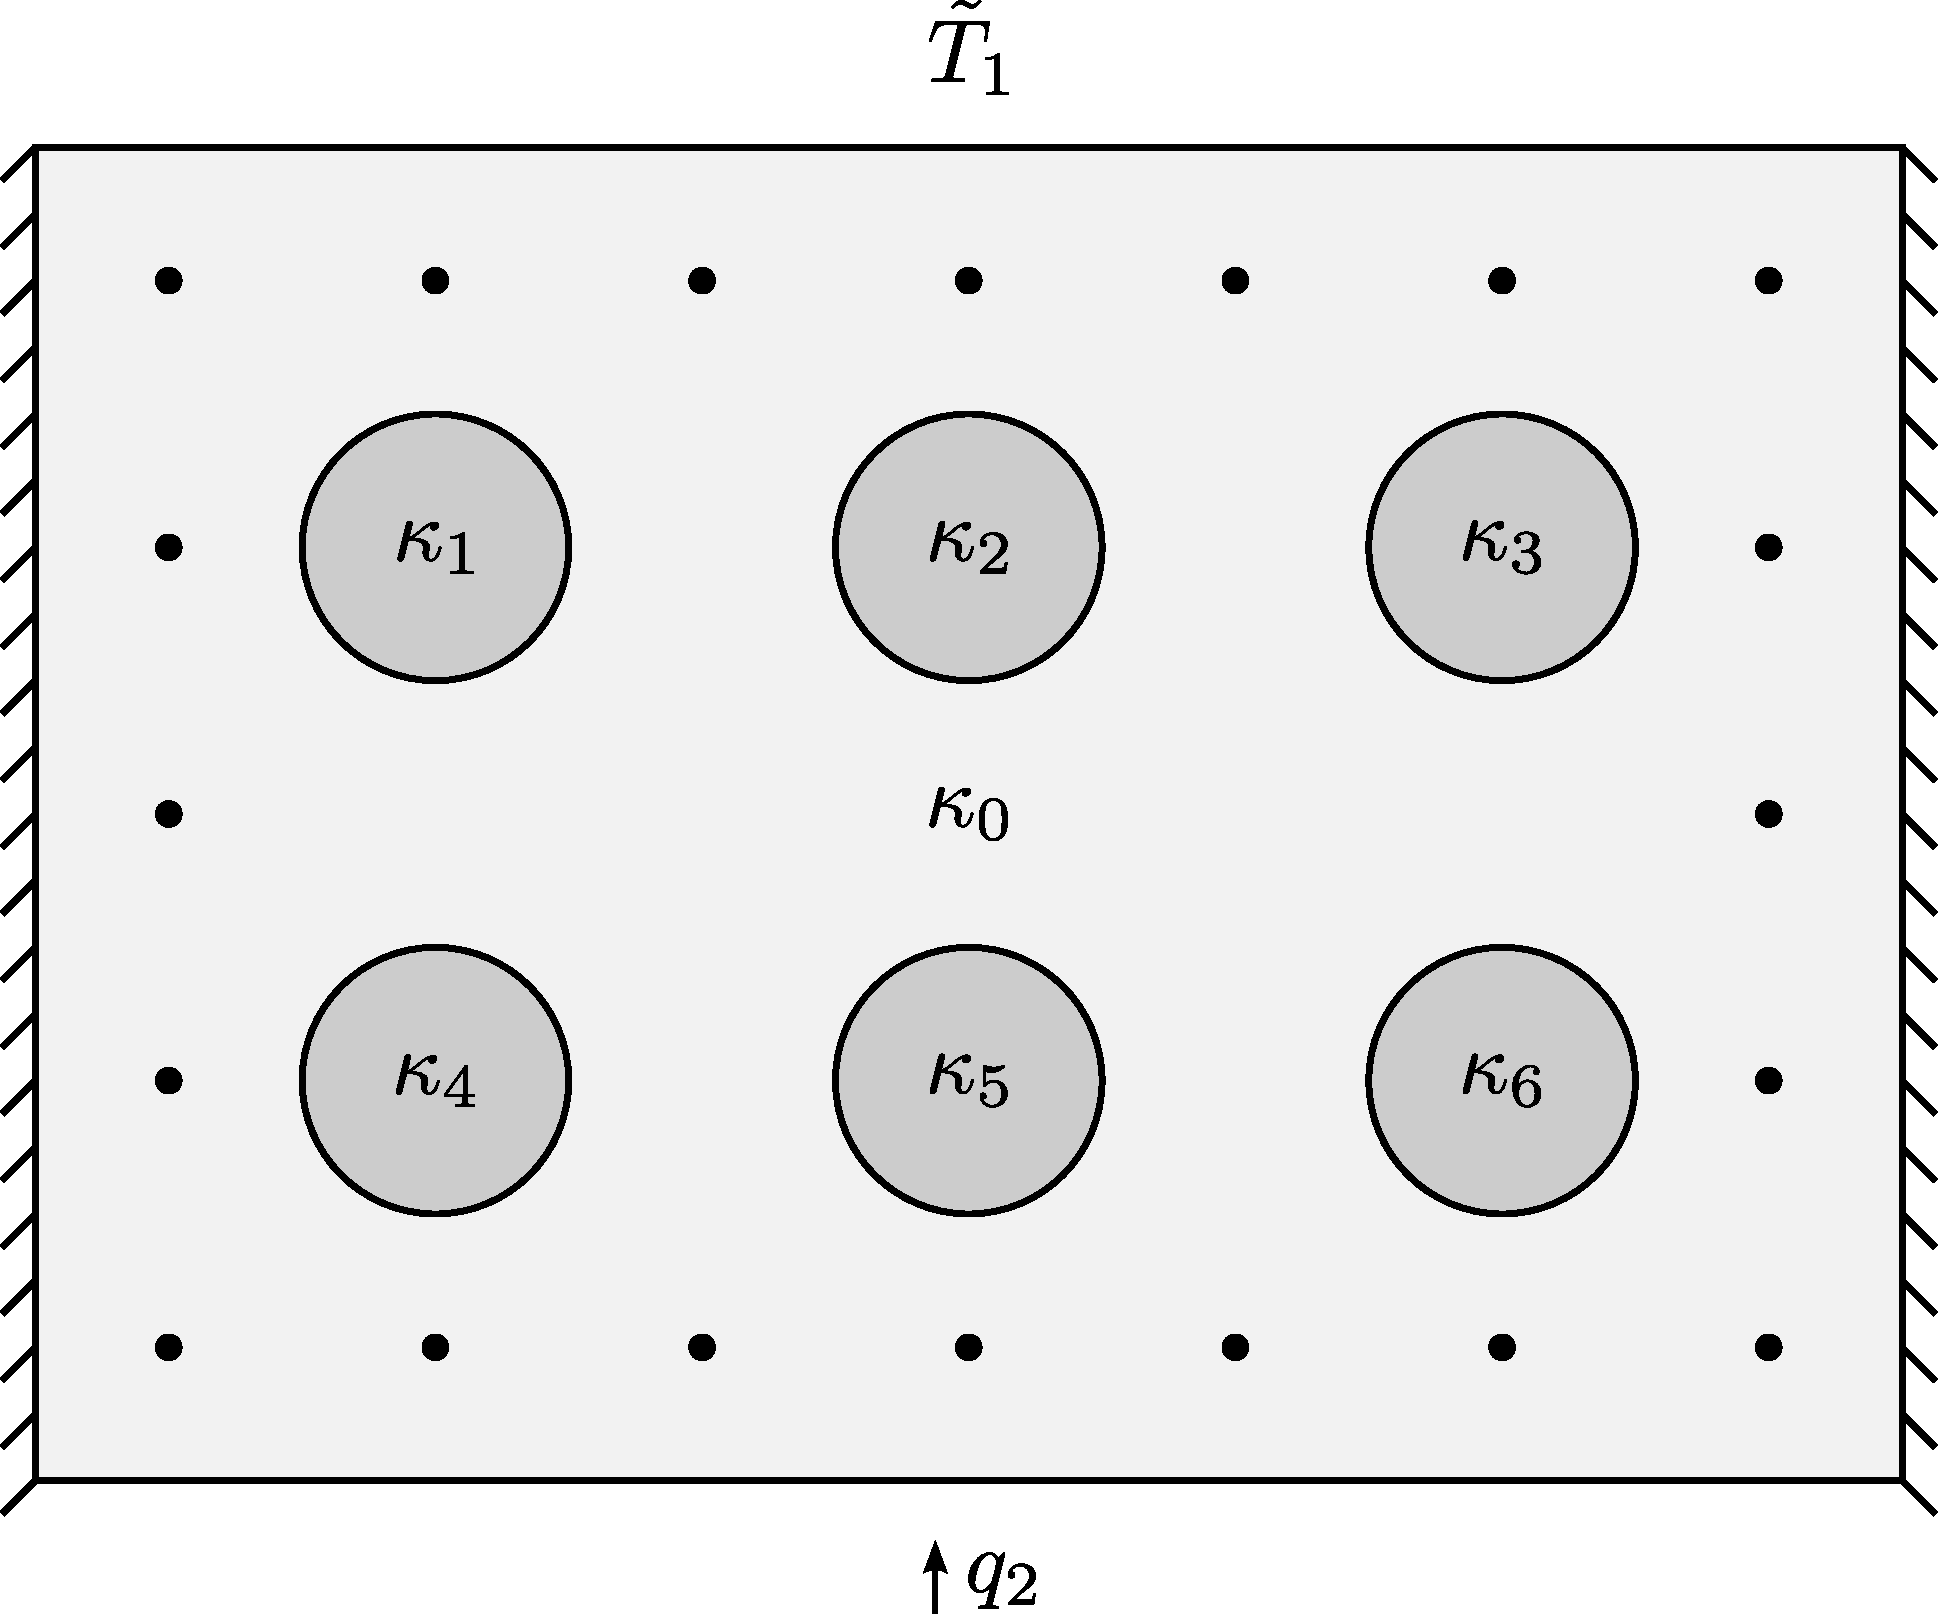
\includegraphics[width=\JCPfemWidth]{fig_JCP_Heat6D_HeatConduction}
  \caption[6D IHCP: Heat conduction setup]{6D IHCP: Heat conduction setup.}
  \label{fig:JCP:Thermal:HeatConduction}
\end{figure}

\subsubsection{Posterior density}
% LIKELIHOOD EXPANSION
The unknowns are represented as \(\kappa_i = \exp(\lambda_0 + \varsigma_0 \xi_i)\) in terms of the standardized variables
\(\xi_i \in \mathds{R}\) with Gaussian weight functions \(\mathcal{N}(\xi_i \cond 0,1)\).
A spectral expansion \(\hat{\mathcal{L}}_p\) in tensorized Hermite polynomials is then computed for \(p = 5\) and \(K = 5 \times 10^4\).
The errors of the likelihood approximation are estimated as \(\epsilon_{\mathrm{Emp}} = 8.81 \times 10^{-1}\) and \(\epsilon_{\mathrm{LOO}} = 9.14 \times 10^{-1}\).
As compared to the low-dimensional examples that were studied before, these are large errors.
% BASELINE CHANGE
An auxiliary reference density \(\newBase(\bm{\kappa}) = \prod_{i=1}^6 \newBase(\kappa_i)\) is then constructed as a
multivariate lognormal with independent marginals \(\newBase(\kappa_i) = \mathcal{LN}(\kappa_i \cond \mu_i,\sigma_i^2)\).
The parameters of the latter are chosen as the means \(\mu_i = \mathds{E}[\kappa_i \cond \bm{T}]\) and standard deviations
\(\sigma_i = \mathrm{Std}[\kappa_i \cond \bm{T}]\) of the posterior surrogate corresponding to the coefficients of SLE \(\hat{\mathcal{L}}_p\).
We remark that this is a simple two-step procedure and that a more refined usage of the reference change would certainly lead to more sophisticated approaches.
Subsequently, an aSLE \(\hat{\auxQuantity}_p\) with \(p = 5\) and  \(K = 5 \times 10^4\) is computed.
The errors amount to \(\epsilon_{\mathrm{Emp}} = 4.81 \times 10^{-1}\) and \(\epsilon_{\mathrm{LOO}} = 6.24 \times 10^{-1}\).
Notwithstanding that these errors are smaller than the corresponding errors of the SLE, they are still large as compared to the previous examples.
Since these errors are now measured with respect to the auxiliary density which is expectedly closer to the true posterior than the prior is,
the aSLE presumably leads to a more accurate posterior surrogate.
\par % 1D MARGINALS
From the previously computed SLE \(\hat{\mathcal{L}}(\bm{\kappa})\) and the aSLE \(\hat{\auxQuantity}_p(\bm{\kappa})\)
approximations of the joint posterior density are computed via \cref{eq:JCP:SLE:Posterior,eq:JCP:SLE:BaselineChange:Posterior}.
The obtained surrogates \(\pi(\bm{\kappa} \cond \bm{T}) \approx \hat{\mathcal{L}}_p(\bm{\kappa}) \pi(\bm{\kappa}) / \coeffL_{\bm{0}}\) and
\(\pi(\bm{\kappa} \cond \bm{T}) \approx \hat{\auxQuantity}_p(\bm{\kappa}) \newBase(\bm{\kappa}) / \coeffBaseL_{\bm{0}}\) are now compared to each other.
We start with the one-dimensional marginals that can be compiled by collecting terms from the full expansions based on \cref{eq:JCP:SLE:Marginal1D}.
For \(j = 1,\ldots,6\) the marginals \(\pi(\kappa_j \cond \bm{T})\) that are extracted that way are shown in \cref{fig:JCP:Thermal:Post1D}.
The marginal priors \(\pi(\kappa_j)\) and the auxiliary densities \(\newBase(\kappa_j)\) are shown, too.
% DISCUSSION
While the marginals that are taken from the SLE slightly deviate from their MCMC counterparts, the marginals based on the aSLE match their references perfectly well.
The reason is that the posterior can be easier represented as a small adjustment of the auxiliary density than as a large correction to the prior.
Thus, with the same expansion order the posterior is more accurately represented through the aSLE than through the SLE.
Regarding the size of the error estimates, it is surprising that the marginals can be retrieved that well with the aSLE.
Even though the SLE-based posterior approximations can hardly be interpreted as proper probability densities, i.e.\ they conspicuously take on negative values,
the moments are recovered sufficiently well for the construction of the auxiliary reference density.
% POSTERIOR MARGINALS
\begin{figure}[htbp]
  \centering
  \begin{subfigure}[b]{\JCPsubWidth}
    \centering
    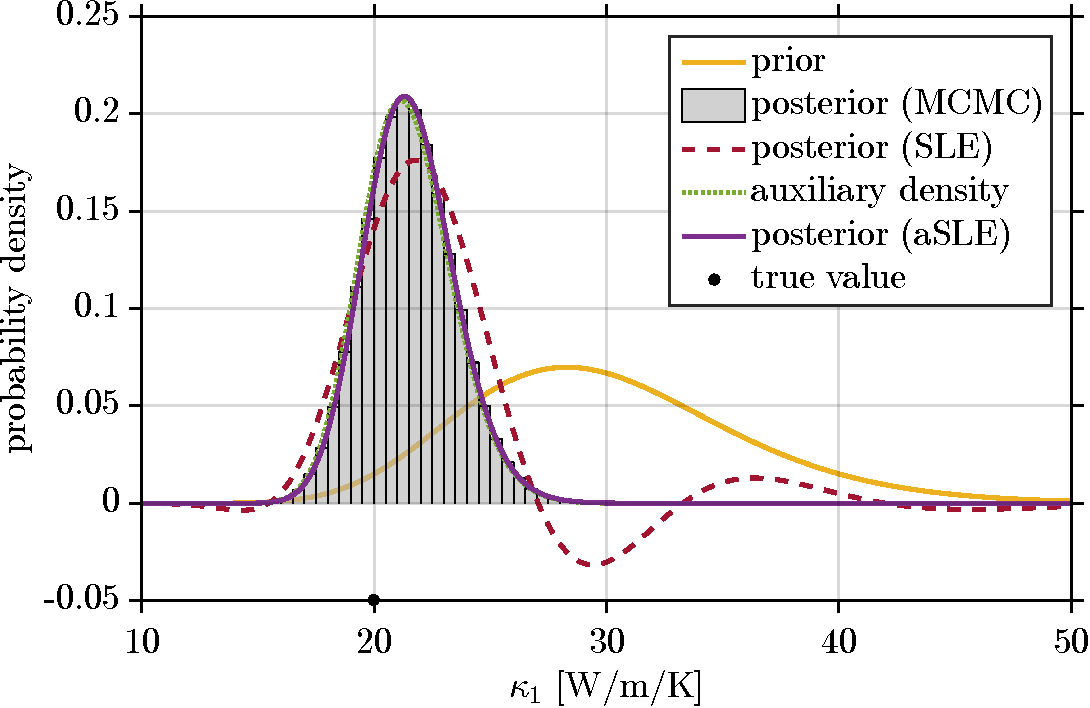
\includegraphics[height=\JCPfigHeight]{fig_JCP_Heat6D_Post1D_k1}
    \caption{Thermal conductivity \(\kappa_1\).}
    \label{fig:JCP:Thermal:Post1D:k1}
  \end{subfigure}\hfill%
  \begin{subfigure}[b]{\JCPsubWidth}
    \centering
    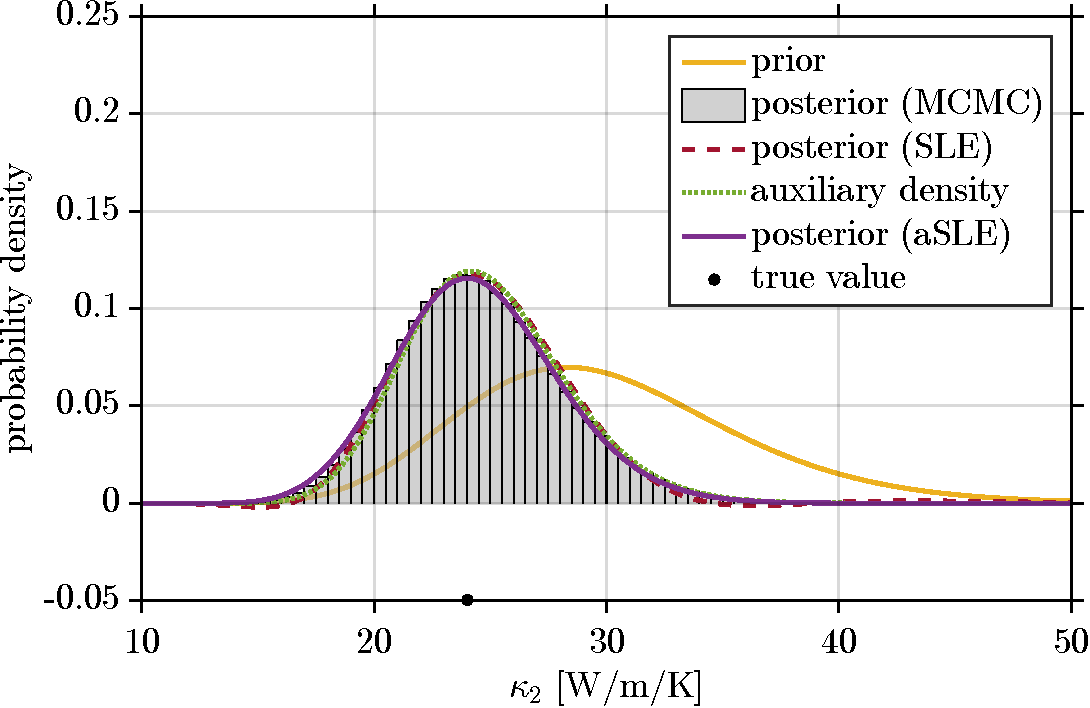
\includegraphics[height=\JCPfigHeight]{fig_JCP_Heat6D_Post1D_k2}
    \caption{Thermal conductivity \(\kappa_2\).}
    \label{fig:JCP:Thermal:Post1D:k2}
  \end{subfigure}\\[3ex]%
  \begin{subfigure}[b]{\JCPsubWidth}
    \centering
    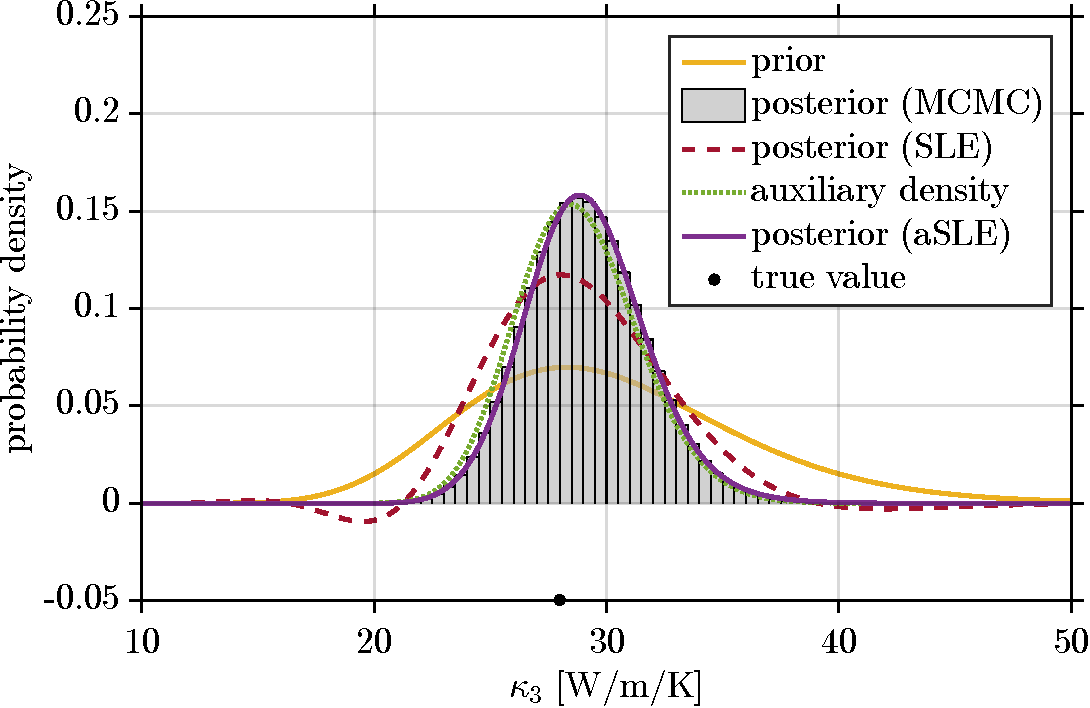
\includegraphics[height=\JCPfigHeight]{fig_JCP_Heat6D_Post1D_k3}
    \caption{Thermal conductivity \(\kappa_3\).}
    \label{fig:JCP:Thermal:Post1D:k3}
  \end{subfigure}\hfill%
  \begin{subfigure}[b]{\JCPsubWidth}
    \centering
    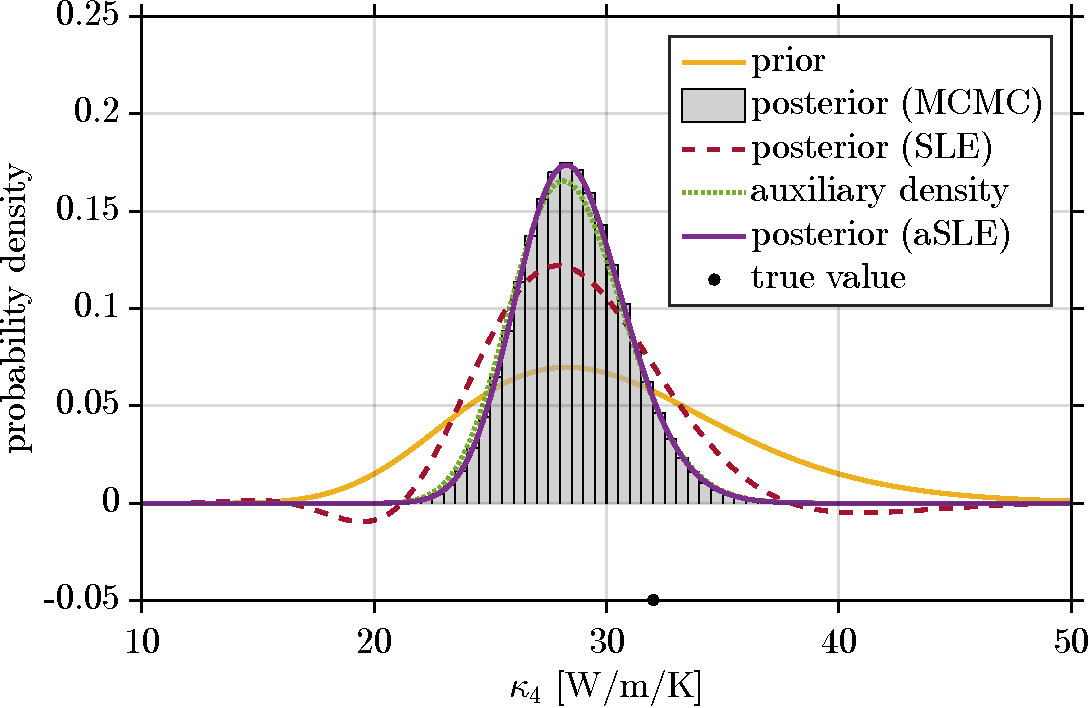
\includegraphics[height=\JCPfigHeight]{fig_JCP_Heat6D_Post1D_k4}
    \caption{Thermal conductivity \(\kappa_4\).}
    \label{fig:JCP:Thermal:Post1D:k4}
  \end{subfigure}\\[3ex]%
  \begin{subfigure}[b]{\JCPsubWidth}
    \centering
    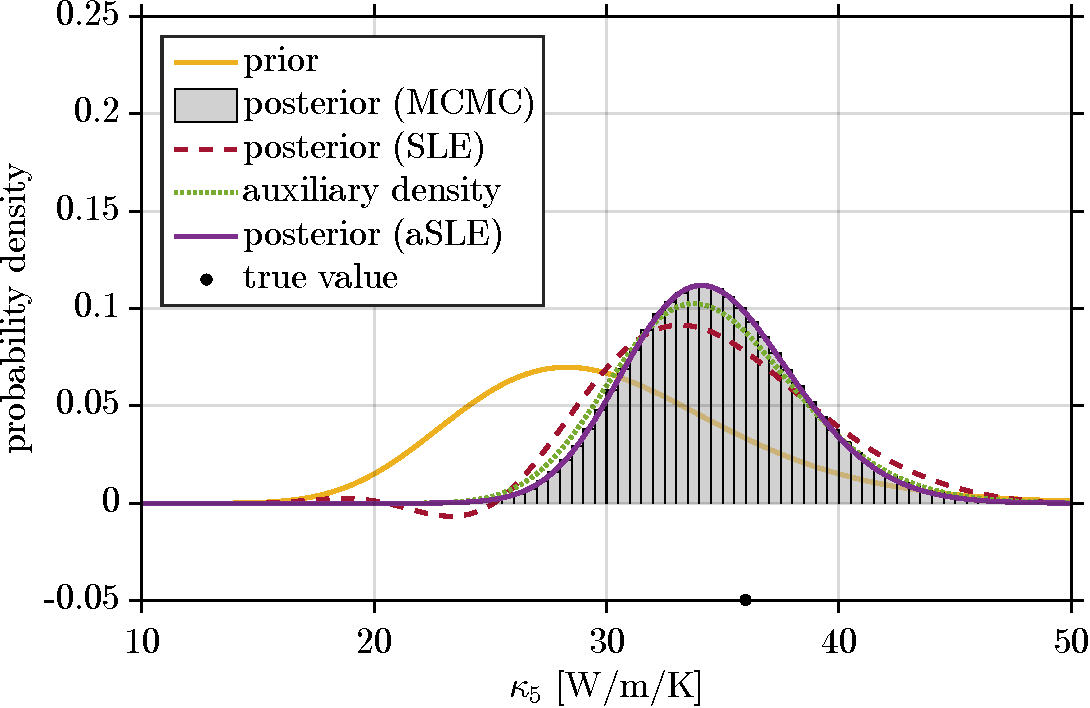
\includegraphics[height=\JCPfigHeight]{fig_JCP_Heat6D_Post1D_k5}
    \caption{Thermal conductivity \(\kappa_5\).}
    \label{fig:JCP:Thermal:Post1D:k5}
  \end{subfigure}\hfill%
  \begin{subfigure}[b]{\JCPsubWidth}
    \centering
    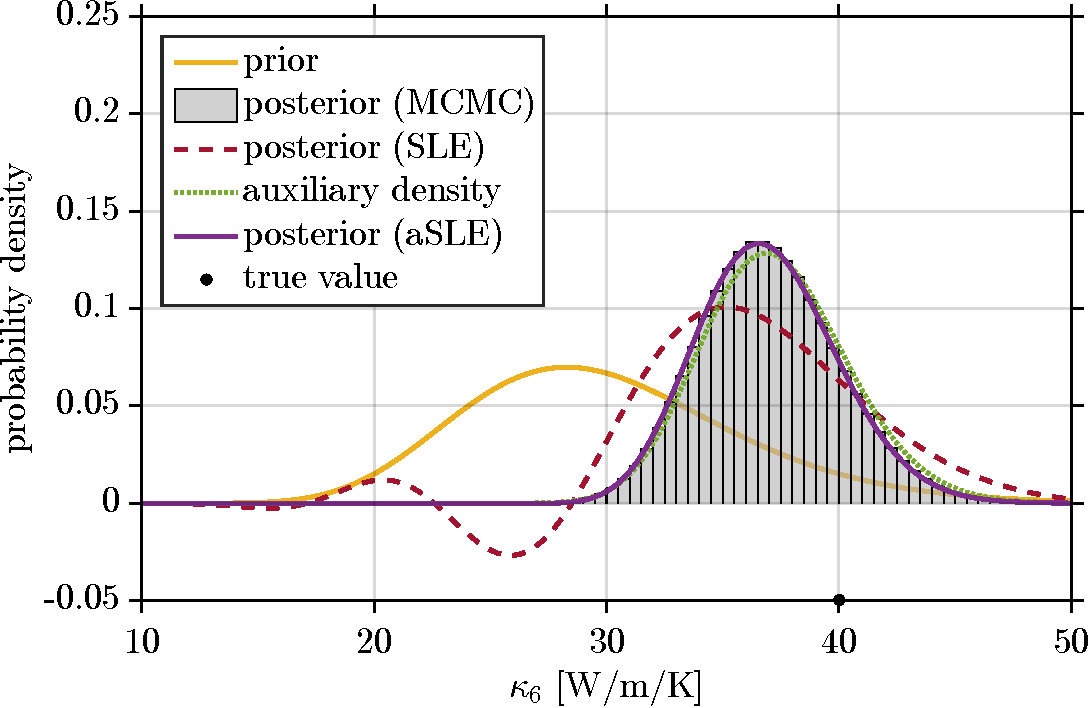
\includegraphics[height=\JCPfigHeight]{fig_JCP_Heat6D_Post1D_k6}
    \caption{Thermal conductivity \(\kappa_6\).}
    \label{fig:JCP:Thermal:Post1D:k6}
  \end{subfigure}%
  \caption[6D IHCP: Posterior marginals]{6D IHCP: Posterior marginals.}
  \label{fig:JCP:Thermal:Post1D}
\end{figure}
\par % 2D MARGINALS
On the basis of \cref{eq:JCP:SLE:Marginal2D} the two-dimensional posterior marginals \(\pi(\kappa_j,\kappa_k \cond \bm{T})\) can be constructed from the full expansions.
For \(j = 3\) and \(k = 4\) the posterior marginal for the SLE \(\hat{\mathcal{L}}_p\) is shown in \cref{fig:JCP:Thermal:Post2D:SLE}.
The same two-dimensional distribution is depicted in \cref{fig:JCP:Thermal:Post2D:aSLE} for the aSLE \(\hat{\auxQuantity}_p\).
A histogram of the MCMC sample is provided in \cref{fig:JCP:Thermal:Post2D:MCMC} as a reference.
As already found in \cref{fig:JCP:Thermal:Post1D:k3,fig:JCP:Thermal:Post1D:k4} for instance,
in \cref{fig:JCP:Thermal:Post2D} the aSLE-based surrogate appears to be almost exact whereas the SLE-based one is flattened out.
Since the aSLE captures the true posterior density more accurately than the SLE, we expect similar findings for the posterior moments.
% FIGURES: 2D POSTERIORS
\begin{figure}[htbp]
  \centering
  \begin{subfigure}[b]{\JCPsubWidth}
    \centering
    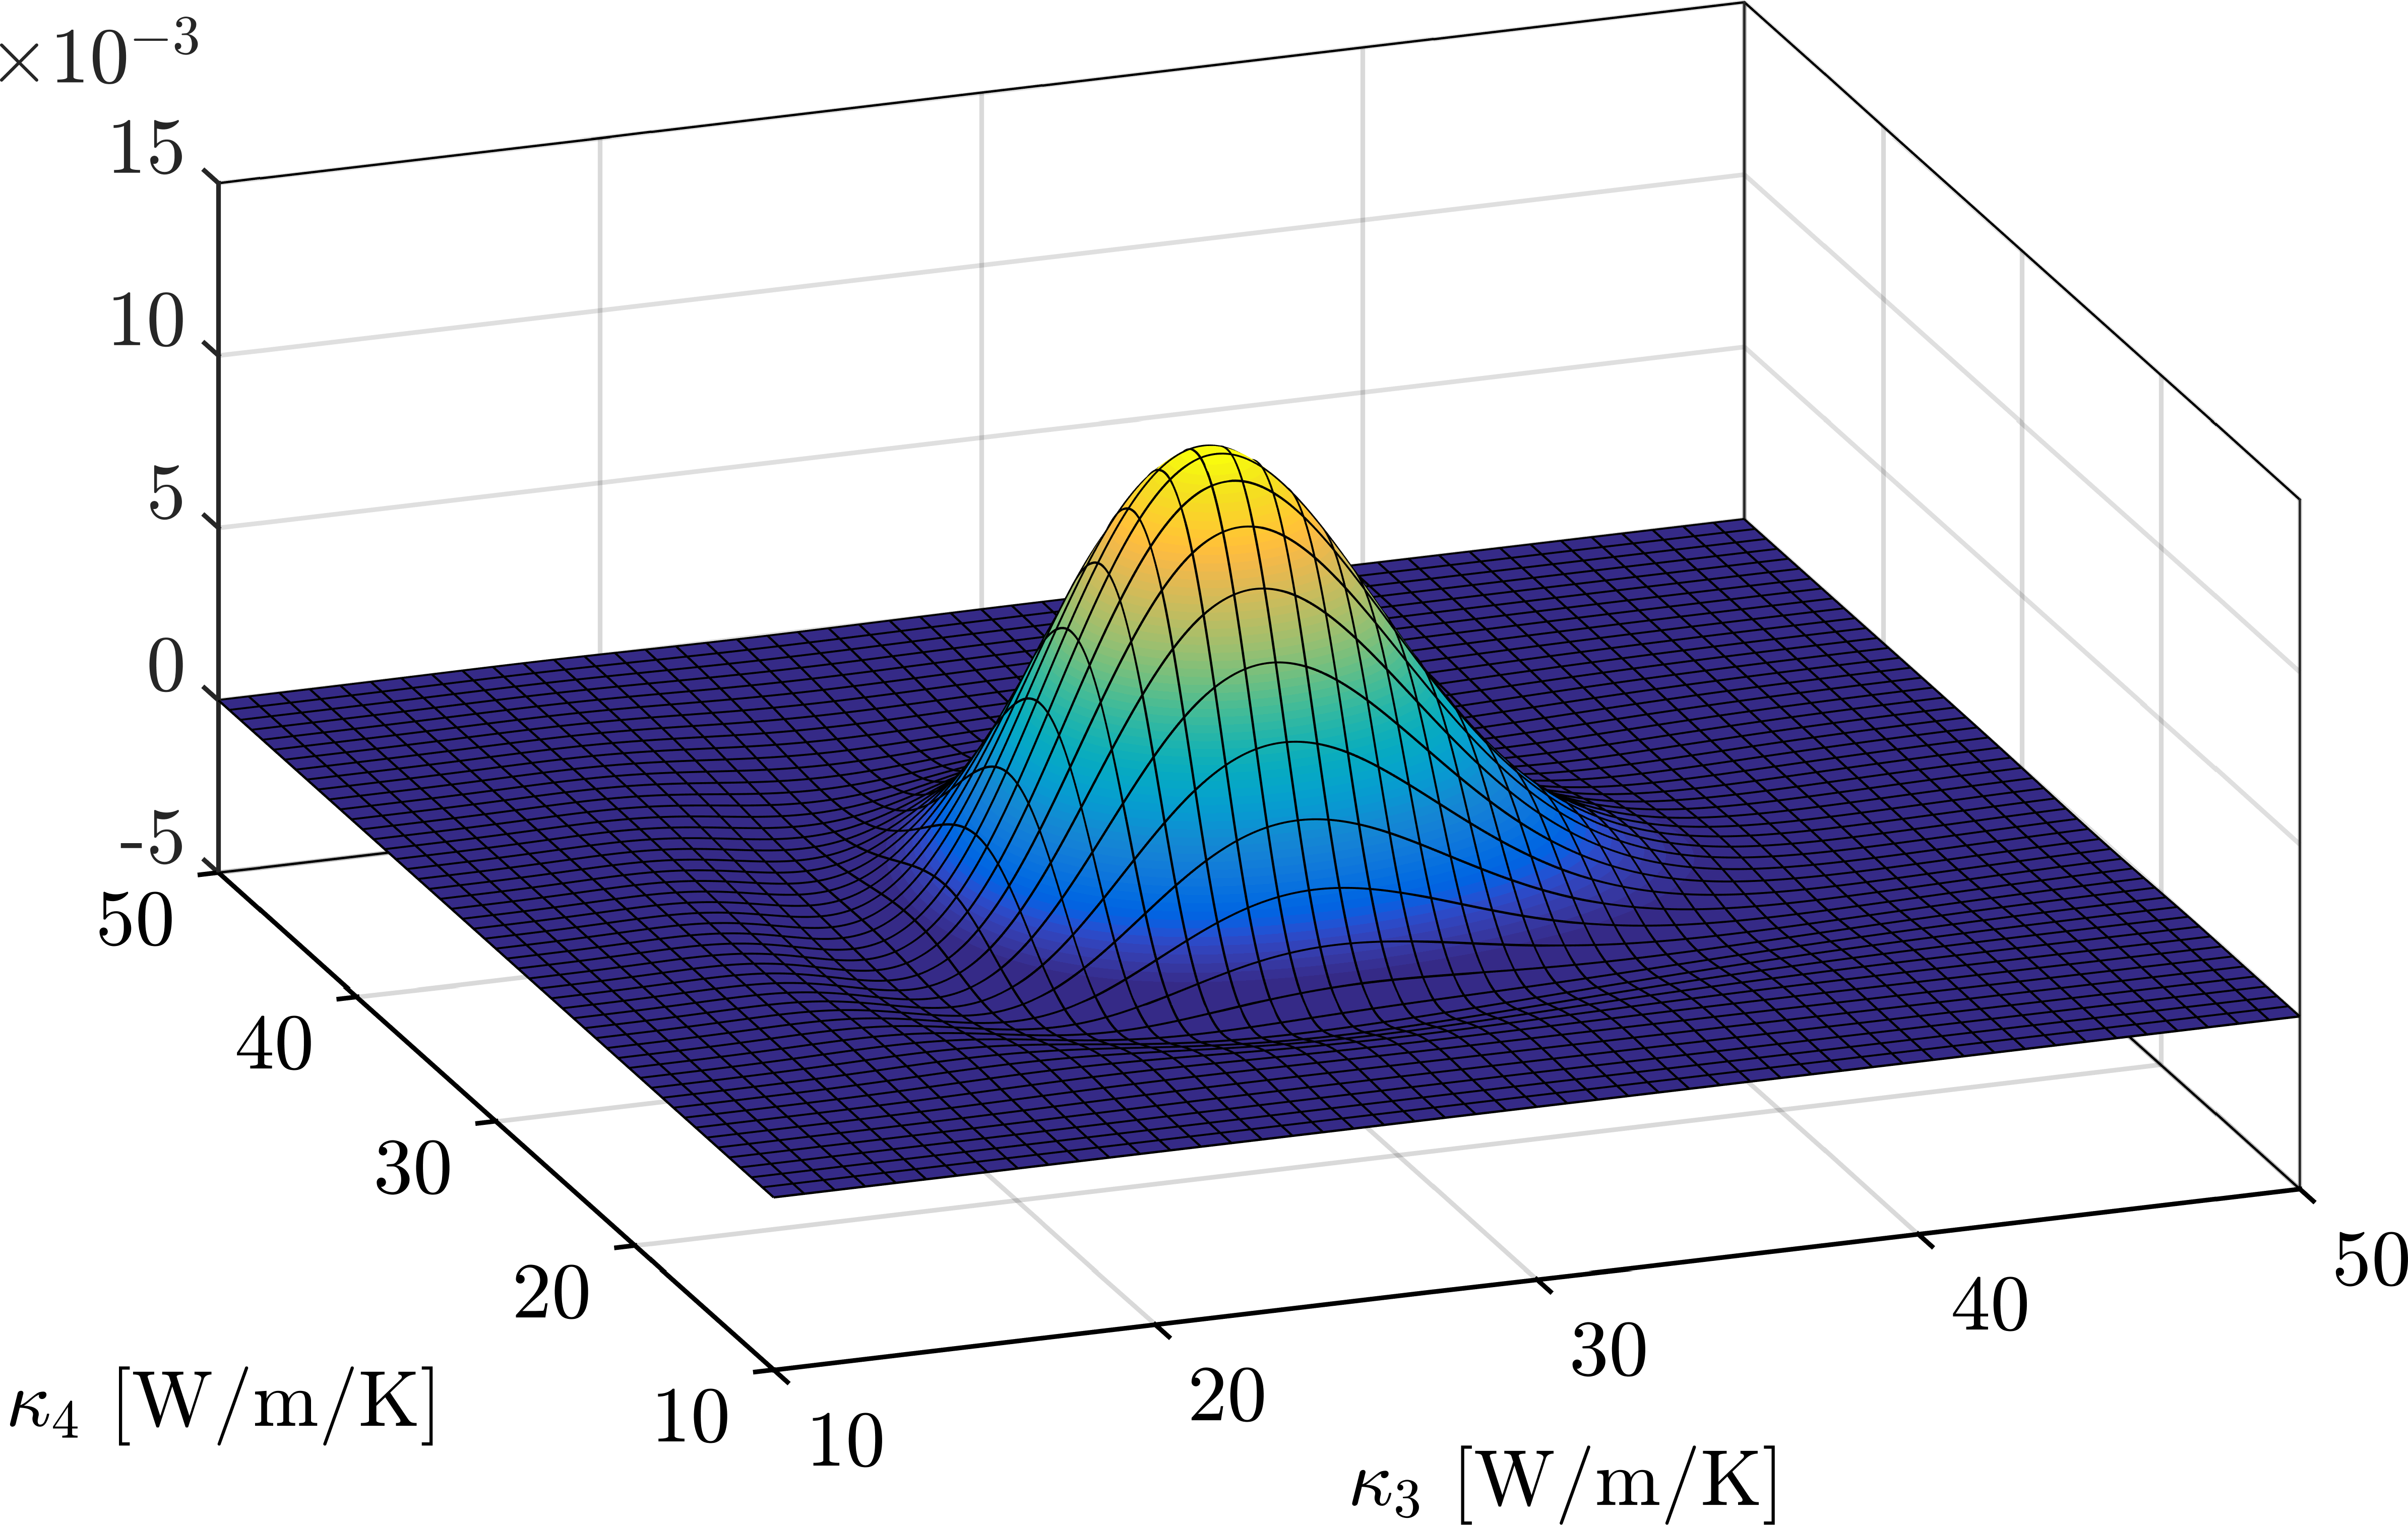
\includegraphics[width=\JCPfigWidth]{fig_JCP_Heat6D_Post2D_SLE}
    \caption{SLE with \(p = 5\).}
    \label{fig:JCP:Thermal:Post2D:SLE}
  \end{subfigure}\hfill%
  \begin{subfigure}[b]{\JCPsubWidth}
    \centering
    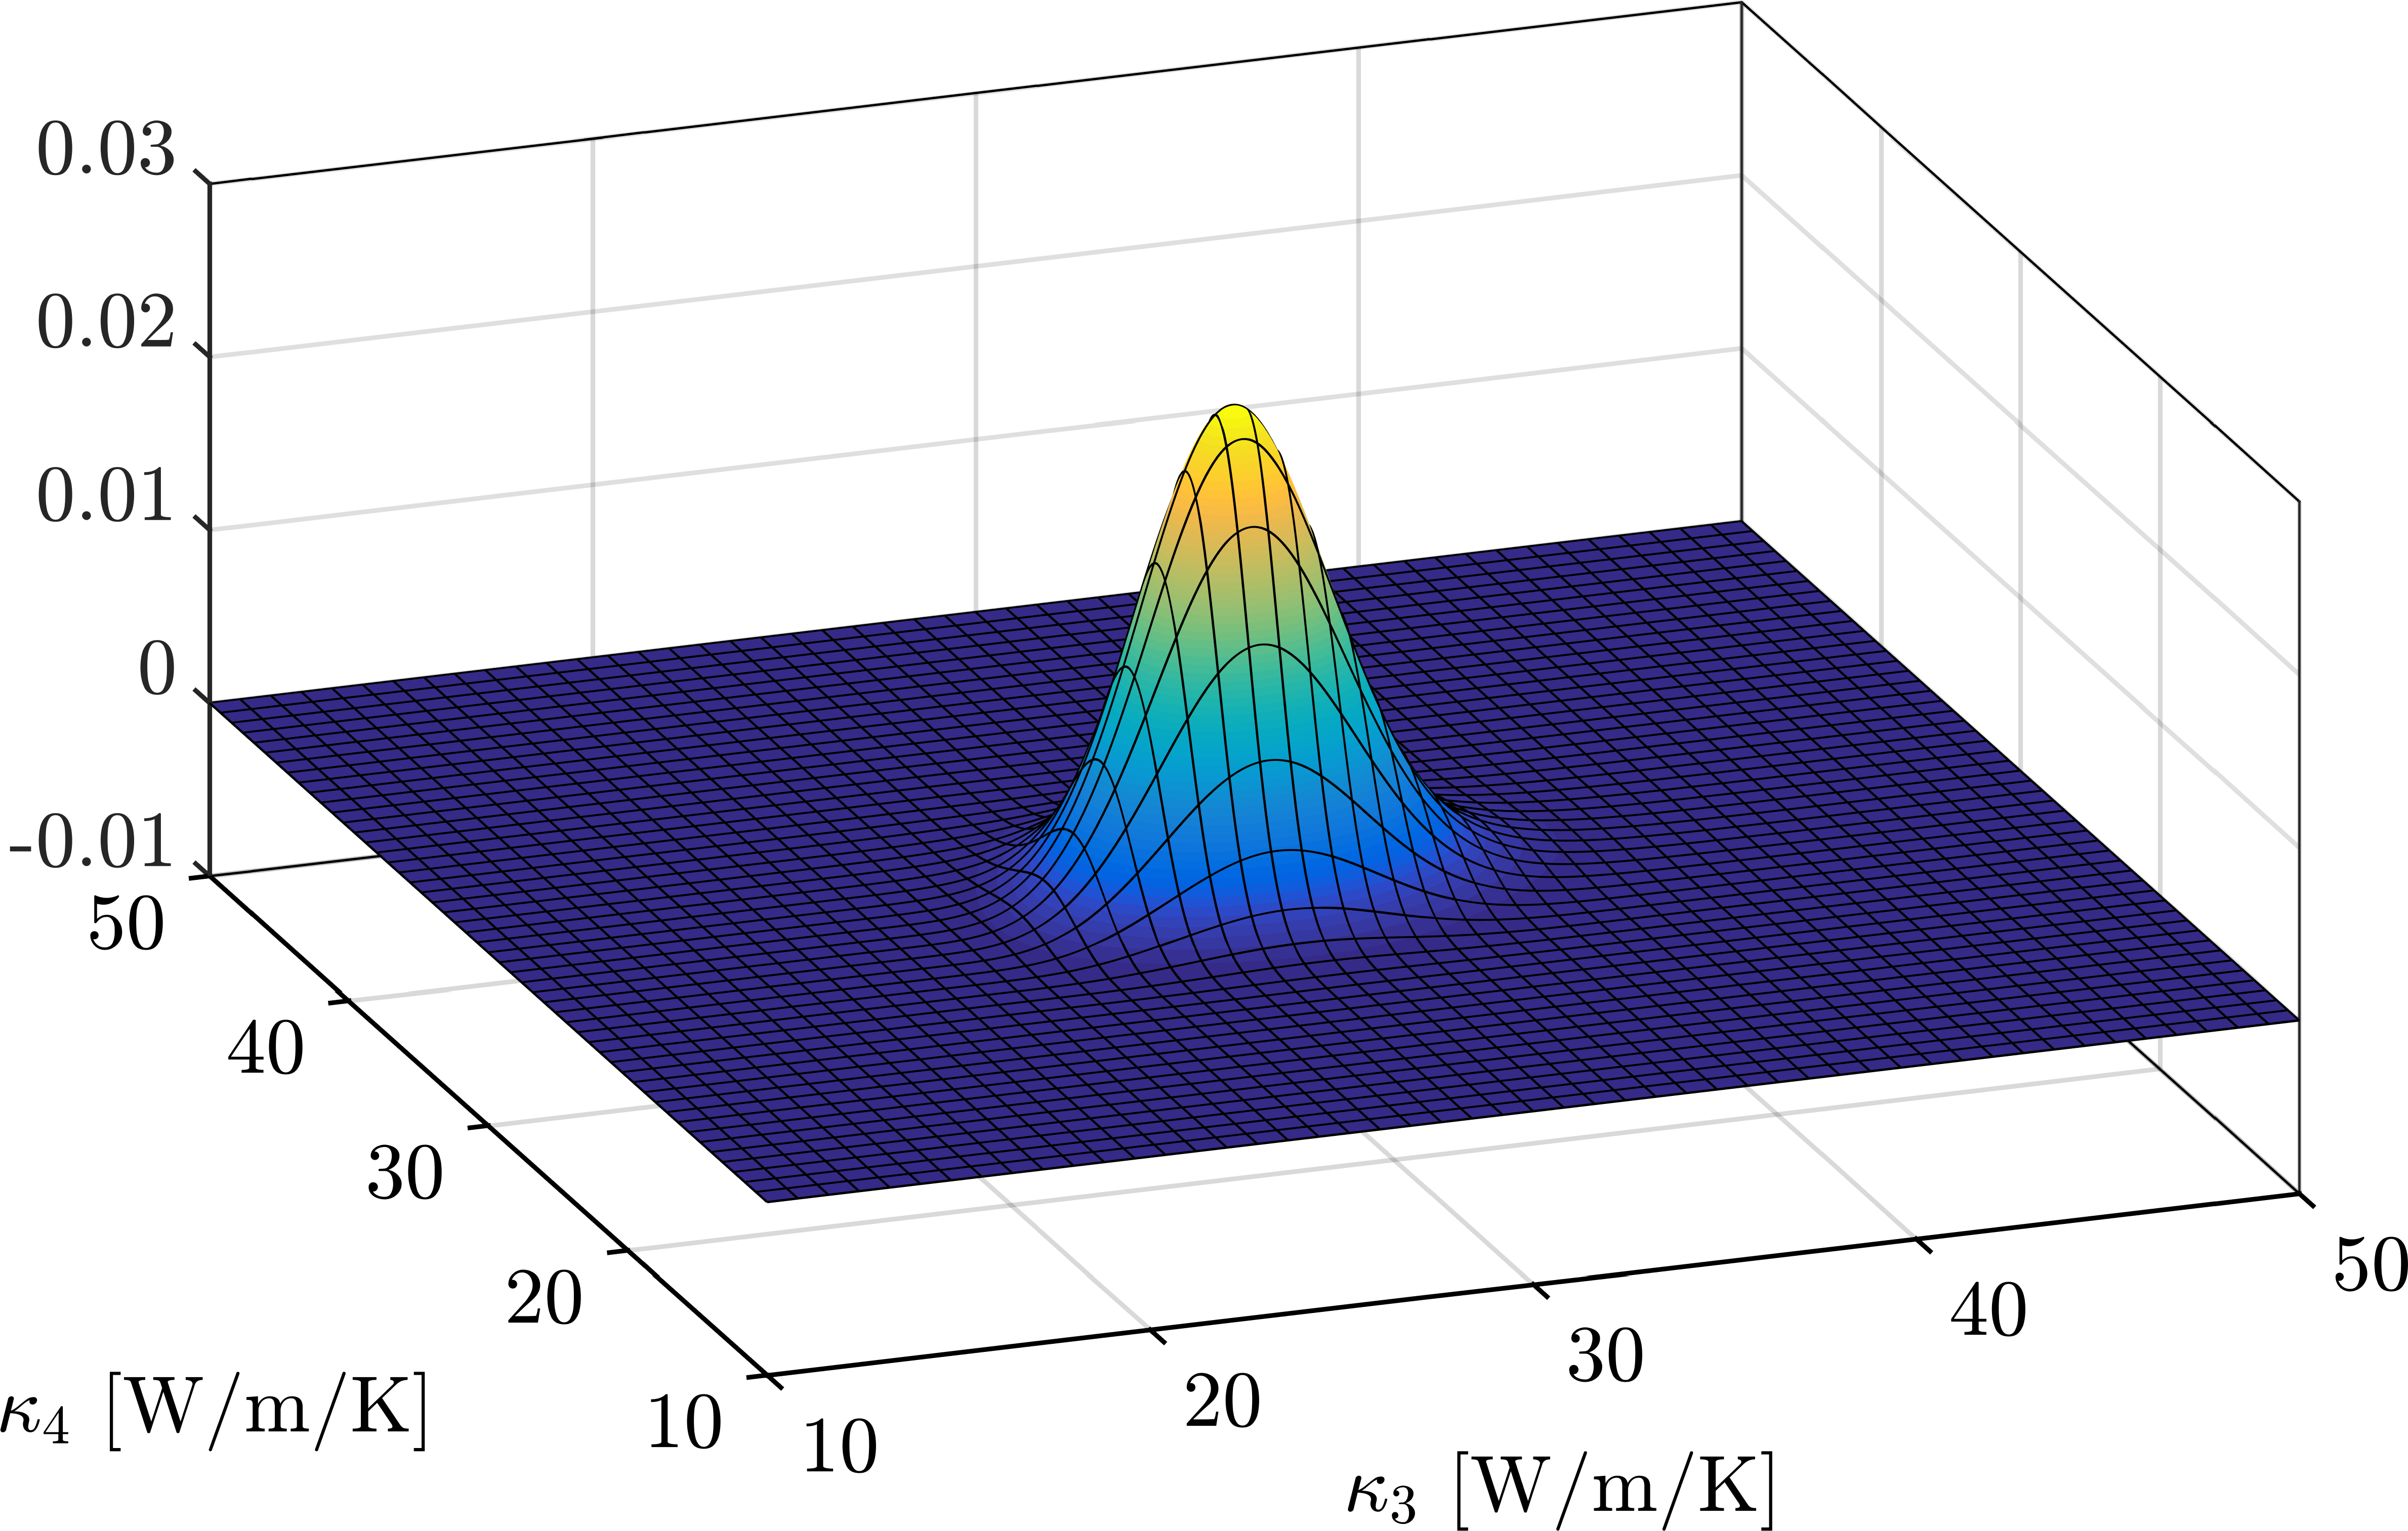
\includegraphics[width=\JCPfigWidth]{fig_JCP_Heat6D_Post2D_aSLE}
    \caption{aSLE with \(p = 5\).}
    \label{fig:JCP:Thermal:Post2D:aSLE}
  \end{subfigure}\\[1ex]%
  \begin{subfigure}[b]{\JCPsubWidth}
    \centering
    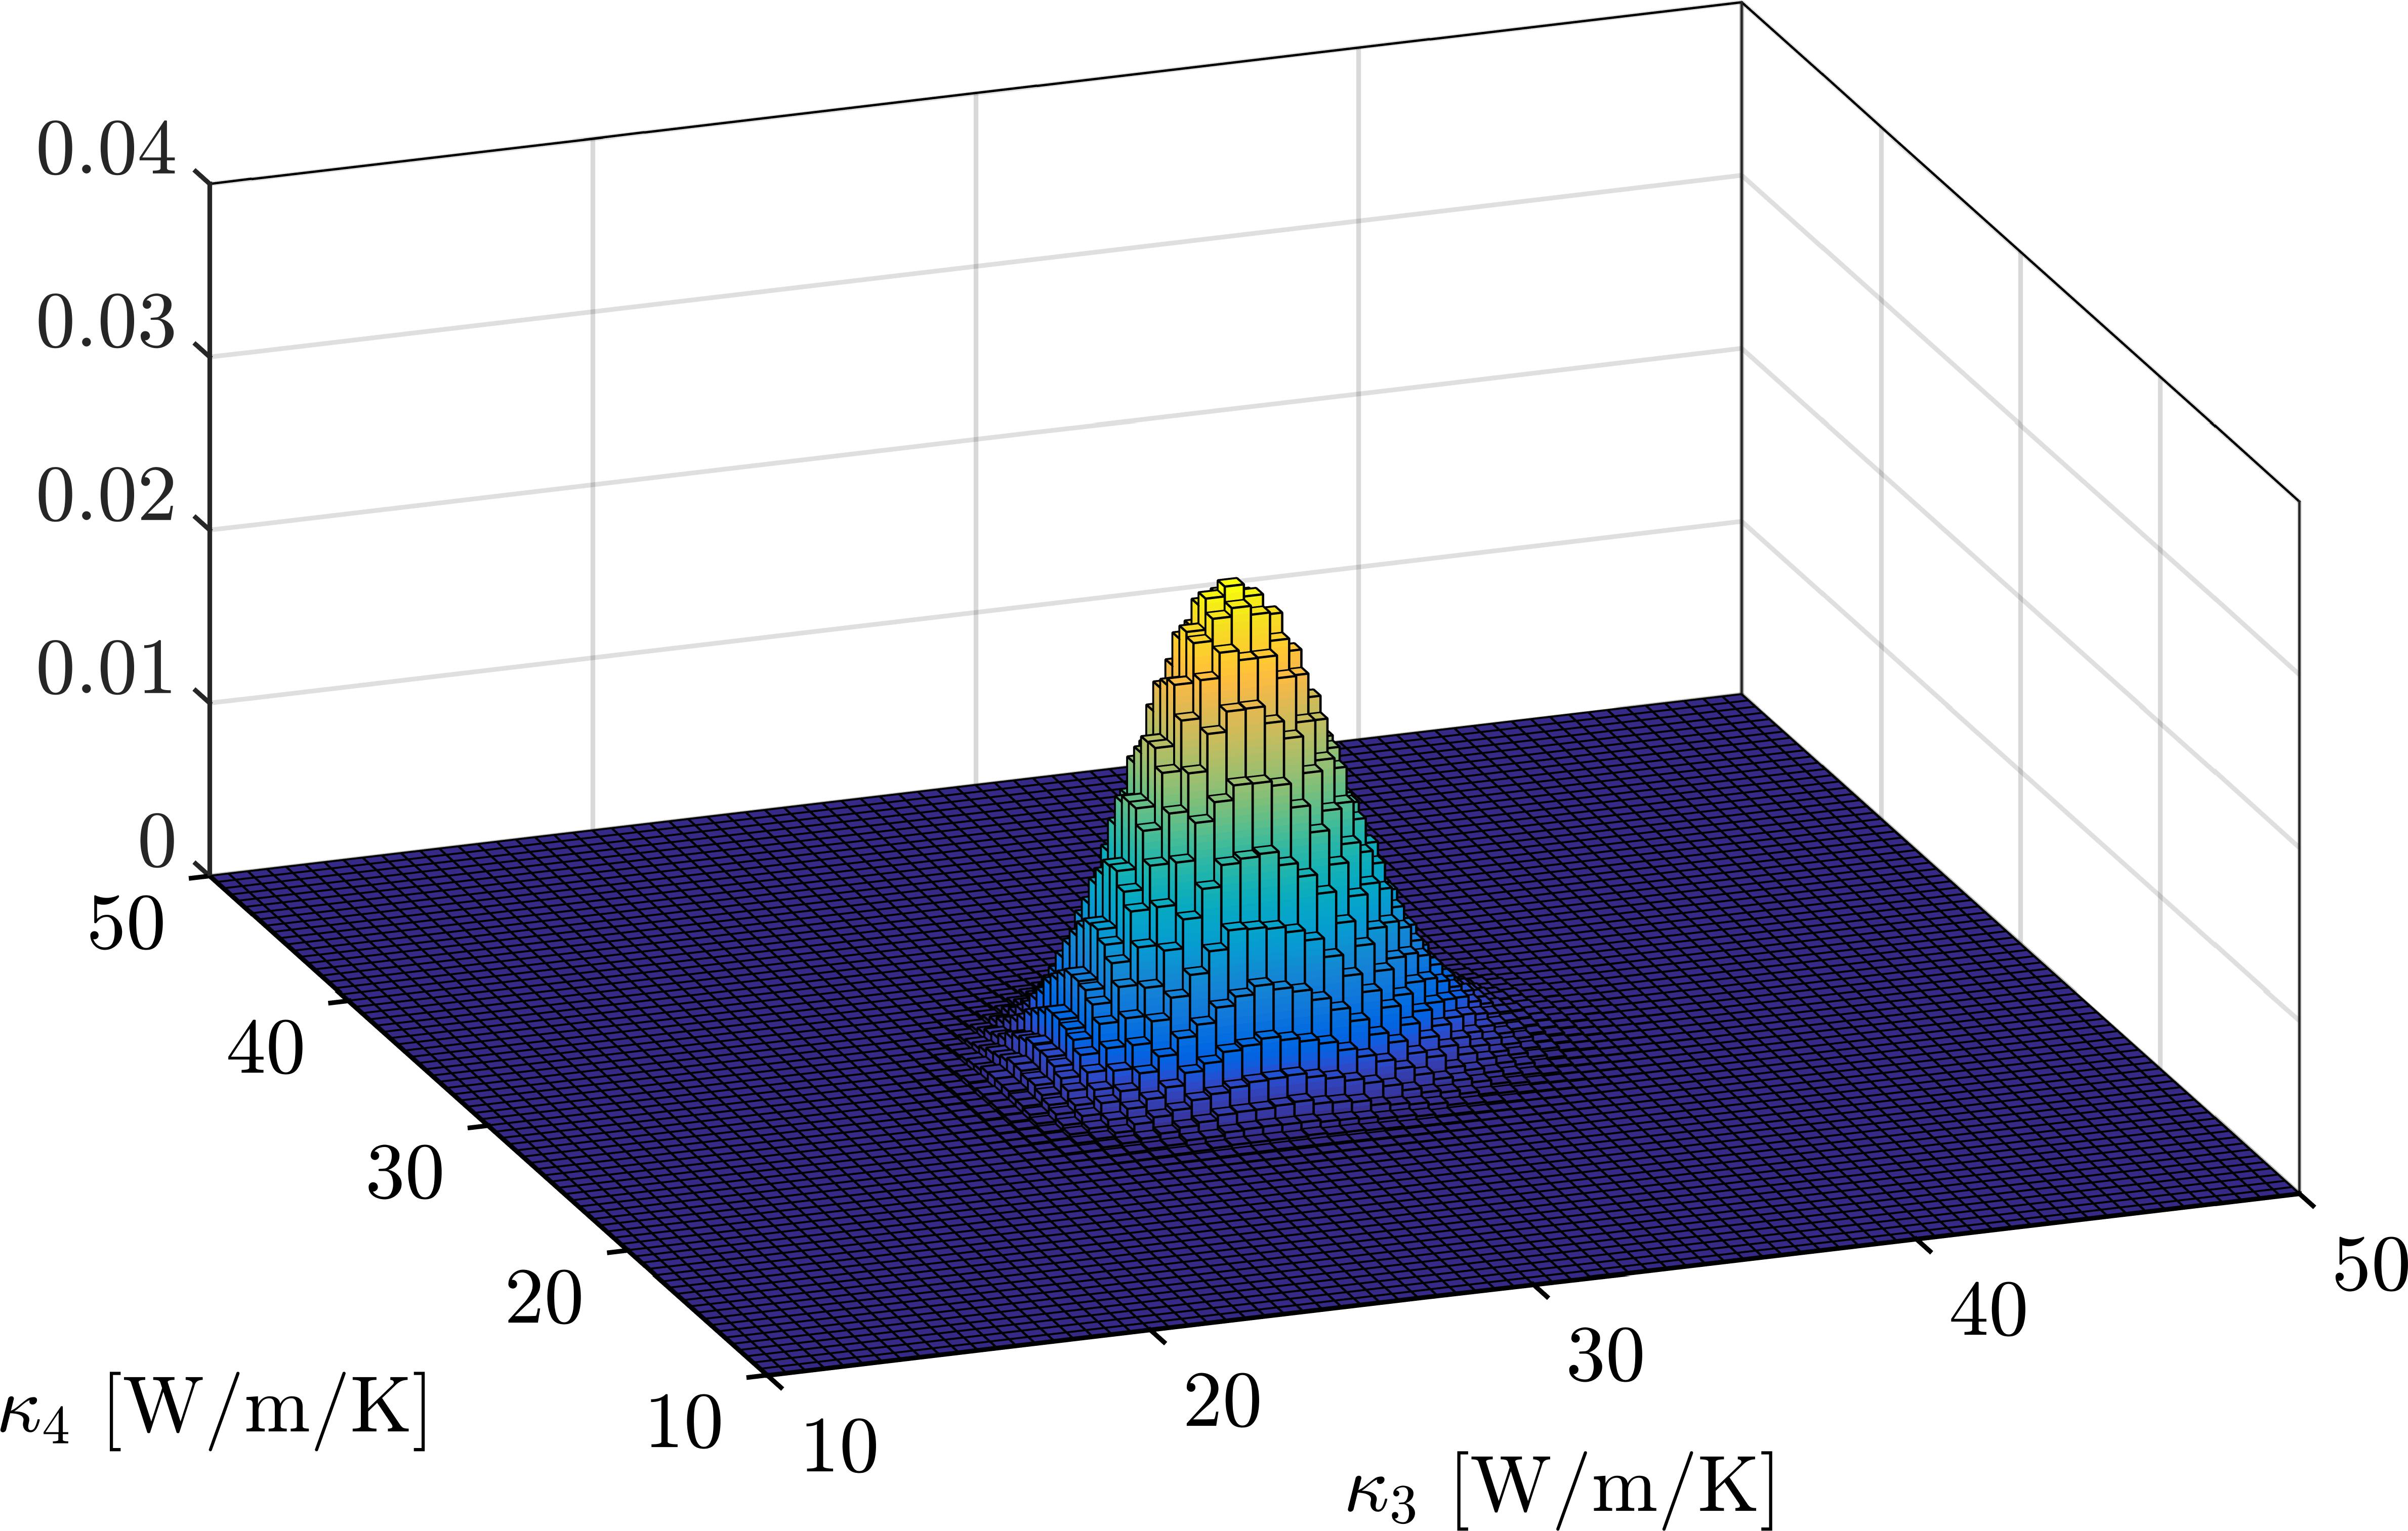
\includegraphics[width=\JCPfigWidth]{fig_JCP_Heat6D_Post2D_MCMC}
    \caption{MCMC reference sample.}
    \label{fig:JCP:Thermal:Post2D:MCMC}
  \end{subfigure}%
  \caption[6D IHCP: Posterior marginals]{6D IHCP: Posterior marginals.}
  \label{fig:JCP:Thermal:Post2D}
\end{figure}

\subsubsection{Quantities of interest}
% STATISTICAL QUANTITIES OF INTEREST
Finally we compute the model evidence and the first posterior moments with the aid of
\cref{eq:JCP:SLE:ScaleFactor,eq:JCP:SLE:BaselineChange:ScaleFactor} and \cref{eq:JCP:SLE:PosteriorMargMean,eq:JCP:SLE:PosteriorMargVariance,eq:JCP:SLE:PosteriorCovariance}.
For the aSLE \(\hat{\auxQuantity}_p\) the analysis proceeds analogously to the SLE \(\hat{\mathcal{L}}_p\).
In \cref{tab:JCP:Thermal:StatisticalQuantities} a summary of the results is given.
As it can be taken from the table, the aSLE consistently gives more accurate estimates of the reference values.
This fulfills our earlier expectations.
Regarding the inaccuracy of the SLE-based posterior marginals and the concerns about interpreting them as probability densities, 
the quality of the SLE-based estimates of the moments surpasses our expectations.
In particular, the estimated standard deviations are more accurate than the surrogate marginals suggest, e.g.\ the ones shown in \cref{fig:JCP:Thermal:Post1D:k1,fig:JCP:Thermal:Post1D:k6}.
Similar as for the posterior density, we have to conclude that the normalized LOO error does not give conclusive information about the accuracy of the first posterior moments.
Nevertheless, it is remarked that the use of resampling methods still ensures a robust fit, i.e.\ it protects against overfitting.
% TABLE: STATISTICAL QUANTITIES
\begin{table}[htbp]
  \caption[6D IHCP: Statistical quantities]{6D IHCP: Statistical quantities.}
  \label{tab:JCP:Thermal:StatisticalQuantities}
  \centering
  \begin{tabular}{rccccccc}
    \toprule
    & \(\scale\) \([10^{-3}]\) & \(\mathds{E}[\kappa_1 \cond \bm{T}]\) & \(\mathds{E}[\kappa_2 \cond \bm{T}]\) & \(\mathds{E}[\kappa_3 \cond \bm{T}]\)
    & \(\mathds{E}[\kappa_4 \cond \bm{T}]\) & \(\mathds{E}[\kappa_5 \cond \bm{T}]\) & \(\mathds{E}[\kappa_6 \cond \bm{T}]\) \\
    \midrule
    SLE    & \(4.04\) & \(21.42\) & \(24.86\) & \(28.79\) & \(28.45\) & \(34.43\) & \(37.27\) \\
    aSLE   & \(3.68\) & \(21.53\) & \(24.48\) & \(29.16\) & \(28.57\) & \(34.59\) & \(36.95\) \\
    (MC)MC & \(3.65\) & \(21.52\) & \(24.57\) & \(29.11\) & \(28.56\) & \(34.64\) & \(37.00\) \\
    \midrule
    & \(\mathrm{Std}[\kappa_1 \cond \bm{T}]\) & \(\mathrm{Std}[\kappa_2 \cond \bm{T}]\) & \(\mathrm{Std}[\kappa_3 \cond \bm{T}]\) & \(\mathrm{Std}[\kappa_4 \cond \bm{T}]\)
    & \(\mathrm{Std}[\kappa_5 \cond \bm{T}]\) & \(\mathrm{Std}[\kappa_6 \cond \bm{T}]\) & \(\rho[\kappa_1,\kappa_2 \cond \bm{T}]\) \\
    \midrule
    SLE    & \(1.95\) & \(3.43\) & \(2.63\) & \(2.43\) & \(3.96\) & \(3.13\) & \(-0.40\) \\
    aSLE   & \(1.94\) & \(3.56\) & \(2.61\) & \(2.33\) & \(3.62\) & \(2.99\) & \(-0.44\) \\
    (MC)MC & \(1.93\) & \(3.48\) & \(2.56\) & \(2.31\) & \(3.64\) & \(3.00\) & \(-0.47\) \\
    \midrule
    & \(\rho[\kappa_1,\kappa_3 \cond \bm{T}]\) & \(\rho[\kappa_1,\kappa_4 \cond \bm{T}]\) & \(\rho[\kappa_1,\kappa_5 \cond \bm{T}]\) & \(\rho[\kappa_1,\kappa_6 \cond \bm{T}]\)
    & \(\rho[\kappa_2,\kappa_3 \cond \bm{T}]\) & \(\rho[\kappa_2,\kappa_4 \cond \bm{T}]\) & \(\rho[\kappa_2,\kappa_5 \cond \bm{T}]\) \\
    \midrule
    SLE    & \(\hphantom{-}0.19\) & \(-0.39\) & \(-0.28\) & \(0.05\) & \(-0.40\) & \(-0.18\) & \(-0.30\) \\ 
    aSLE   & \(-0.01\) & \(-0.29\) & \(-0.03\) & \(0.10\) & \(-0.48\) & \(-0.17\) & \(-0.28\) \\
    (MC)MC & \(-0.02\) & \(-0.32\) & \(-0.03\) & \(0.09\) & \(-0.48\) & \(-0.17\) & \(-0.31\) \\
    \midrule
    & \(\rho[\kappa_2,\kappa_6 \cond \bm{T}]\) & \(\rho[\kappa_3,\kappa_4 \cond \bm{T}]\) & \(\rho[\kappa_3,\kappa_5 \cond \bm{T}]\) & \(\rho[\kappa_3,\kappa_6 \cond \bm{T}]\)
    & \(\rho[\kappa_4,\kappa_5 \cond \bm{T}]\) & \(\rho[\kappa_4,\kappa_6 \cond \bm{T}]\) & \(\rho[\kappa_5,\kappa_6 \cond \bm{T}]\) \\
    \midrule
    SLE    & \(-0.09\) & \(-0.00\) & \(\hphantom{-}0.22\) & \(-0.22\) & \(-0.20\) & \(0.24\) & \(-0.11\) \\
    aSLE   & \(-0.13\) & \(\hphantom{-}0.11\) & \(-0.02\) & \(-0.32\) & \(-0.24\) & \(0.13\) & \(-0.24\) \\
    (MC)MC & \(-0.16\) & \(\hphantom{-}0.10\) & \(-0.03\) & \(-0.34\) & \(-0.26\) & \(0.12\) & \(-0.24\) \\
    \bottomrule
  \end{tabular}
\end{table}